\documentclass[12pt]{article}

%%%%%%%%%%%%%%%%%%%%%%%%%%%%%%%%%%%%%%%%%%%%%%%%%%%%%%%%%%%%%%%%%%%%%%%%%%%%%%%%
%                           Package preset for homework
%%%%%%%%%%%%%%%%%%%%%%%%%%%%%%%%%%%%%%%%%%%%%%%%%%%%%%%%%%%%%%%%%%%%%%%%%%%%%%%%
% Miscellaneous
\usepackage[margin=1in]{geometry}
\usepackage[utf8]{inputenc}
\usepackage{indentfirst}
\usepackage{blindtext}
\usepackage{graphicx}
\usepackage{xr-hyper}
\usepackage{hyperref}
\usepackage{enumitem}
\usepackage{color}
\usepackage{float}
% Math
\usepackage{latexsym}
\usepackage{amsfonts}
\usepackage{amssymb}
\usepackage{amsmath}
\usepackage{commath}
\usepackage{amsthm}
\usepackage{bbold}
\usepackage{bm}
% Physics
\usepackage{physics}
\usepackage{siunitx}
% Code typesetting
\usepackage{listings}
% Citation
\usepackage[authoryear]{natbib}
\usepackage{appendix}
\usepackage[capitalize]{cleveref}
% Title & name
\title{Homework}
\author{Tien Vo}
\date{\today}


%%%%%%%%%%%%%%%%%%%%%%%%%%%%%%%%%%%%%%%%%%%%%%%%%%%%%%%%%%%%%%%%%%%%%%%%%%%%%%%%
%                   User-defined commands and environments
%%%%%%%%%%%%%%%%%%%%%%%%%%%%%%%%%%%%%%%%%%%%%%%%%%%%%%%%%%%%%%%%%%%%%%%%%%%%%%%%
%%% Misc
\sisetup{load-configurations=abbreviations}
\newcommand{\due}[1]{\date{Due: #1}}
\newcommand{\hint}{\textit{Hint}}
\let\oldt\t
\renewcommand{\t}[1]{\text{#1}}

%%% Bold sets & abbrv
\newcommand{\N}{\mathbb{N}}
\newcommand{\Z}{\mathbb{Z}}
\newcommand{\R}{\mathbb{R}}
\newcommand{\Q}{\mathbb{Q}}
\let\oldP\P
\renewcommand{\P}{\mathbb{P}}
\newcommand{\LL}{\mathcal{L}}
\newcommand{\FF}{\mathcal{F}}
\newcommand{\HH}{\mathcal{H}}
\newcommand{\NN}{\mathcal{N}}
\newcommand{\ZZ}{\mathcal{Z}}
\newcommand{\RN}[1]{\textup{\uppercase\expandafter{\romannumeral#1}}}
\newcommand{\ua}{\uparrow}
\newcommand{\da}{\downarrow}

%%% Unit vectors
\newcommand{\xhat}{\vb{\hat{x}}}
\newcommand{\yhat}{\vb{\hat{y}}}
\newcommand{\zhat}{\vb{\hat{z}}}
\newcommand{\nhat}{\vb{\hat{n}}}
\newcommand{\rhat}{\vb{\hat{r}}}
\newcommand{\phihat}{\bm{\hat{\phi}}}
\newcommand{\thetahat}{\bm{\hat{\theta}}}

%%% Other math stuff
\providecommand{\units}[1]{\,\ensuremath{\mathrm{#1}}\xspace}
% Set new style for problem
\newtheoremstyle{problemstyle}  % <name>
        {10pt}                   % <space above>
        {10pt}                   % <space below>
        {\normalfont}           % <body font>
        {}                      % <indent amount}
        {\bfseries\itshape}     % <theorem head font>
        {\normalfont\bfseries:} % <punctuation after theorem head>
        {.5em}                  % <space after theorem head>
        {}                      % <theorem head spec (can be left empty, 
                                % meaning `normal')>

% Set problem environment
\theoremstyle{problemstyle}
\newtheorem{problemenv}{Problem}[section]
\newenvironment{problem}[1]{%
  \renewcommand\theproblemenv{#1}%
  \problemenv
}{\endproblemenv}
% Set lemma environment
\newenvironment{lemma}[2][Lemma]{\begin{trivlist}
\item[\hskip \labelsep {\bfseries #1}\hskip \labelsep {\bfseries #2.}]}{\end{trivlist}}
% Set solution environment
\newenvironment{solution}{
    \begin{proof}[Solution]$ $\par\nobreak\ignorespaces
}{\end{proof}}
\numberwithin{equation}{problemenv}

%%% Page format
\setlength{\parindent}{0.5cm}
\setlength{\oddsidemargin}{0in}
\setlength{\textwidth}{6.5in}
\setlength{\textheight}{8.8in}
\setlength{\topmargin}{0in}
\setlength{\headheight}{18pt}

%%% Code environments
\definecolor{dkgreen}{rgb}{0,0.6,0}
\definecolor{gray}{rgb}{0.5,0.5,0.5}
\definecolor{mauve}{rgb}{0.58,0,0.82}
\lstset{frame=tb,
  language=Python,
  aboveskip=3mm,
  belowskip=3mm,
  showstringspaces=false,
  columns=flexible,
  basicstyle={\small\ttfamily},
  numbers=none,
  numberstyle=\tiny\color{gray},
  keywordstyle=\color{blue},
  commentstyle=\color{dkgreen},
  stringstyle=\color{mauve},
  breaklines=true,
  breakatwhitespace=true,
  tabsize=4
}
\lstset{
  language=Mathematica,
  numbers=left,
  numberstyle=\tiny\color{gray},
  numbersep=5pt,
  breaklines=true,
  captionpos={t},
  frame={lines},
  rulecolor=\color{black},
  framerule=0.5pt,
  columns=flexible,
  tabsize=2
}


\title{Homework 9: Phys 7320 (Spring 2022)}
\due{March 30, 2022}

\begin{document}
\maketitle
%%%%%%%%%%%%%%%%%%%%%%%%%%%%%%%%%%%%%%%%%%%%%%%%%%%%%%%%%%%%%%%%%%%%%%%%%%%%%%%
\begin{problem}{9.1}[Relativistic particle in electric field]
A particle with mass $m$ and charge $e$ moves in a uniform, static, electric
field $\vb{E}_0$.

(a) Solve for the velocity and position of the particle as explicit functions of
time, assuming that the initial velocity $\vb{v}_0$ was perpendicular to the
electric field.

(b) Eliminate the time to obtain the trajectory of the particle in space.
Discuss the shape of the path for short and long times (define ``short'' and
``long'' times).
\begin{solution}
(a) First, we write down the field-strength tensor
\begin{equation}
    F^{\alpha\beta}=\mqty(0&-E_0&0&0\\E_0&0&0&0\\0&0&0&0\\0&0&0&0).
\end{equation}
Then the force equation is
\begin{equation}
    \frac{dU^{\alpha}}{d\tau}
    =\frac{e}{mc}F^{\alpha\beta}U_\beta
    =\frac{eE_0}{mc}\mqty(0&-1&0&0\\1&0&0&0\\0&0&0&0\\0&0&0&0)
    \mqty(U^0\\-U^1\\-U^2\\-U^3)
    =\frac{eE_0}{mc}\mqty(U^1\\U^0\\0\\0).
\end{equation}
It then follows that
\begin{equation}
    \frac{d^2U^0}{d\tau^2}=\qty(\frac{eE_0}{mc})^2U^0,\qquad
    \frac{d^2U^1}{d\tau^2}=\qty(\frac{eE_0}{mc})^2U^1,\qquad\t{and}\qquad
    \frac{dU^2}{d\tau}=\frac{dU^3}{d\tau}=0.
\end{equation}
The problem essentially becomes 2-dimensional, since the $z$ dimension is
ignorable. At $t=0$, $U^2=\gamma_0v_0$ where $\gamma_0=1/\sqrt{1-v_0^2/c^2}$.
Thus, $u_y=(\gamma_0/\gamma)v_0$. The general solution for the differential
equations in $U^0$ and $U^1$ is
\begin{subequations}
    \begin{align}
        c\gamma=U^0
        &=A\sinh\qty(\frac{eE_0\tau}{mc})+B\cosh\qty(\frac{eE_0\tau}{mc}) \\
        \gamma u_x=U^1&
        =\frac{mc}{eE_0}\frac{dU^0}{d\tau}
        =A\cosh\qty(\frac{eE_0\tau}{mc})+B\sinh\qty(\frac{eE_0\tau}{mc}).
    \end{align} 
\end{subequations}
Using initial conditions $U^0(\tau=0)=c\gamma_0$ and $U^1(\tau=0)=0$, we can
write
\begin{subequations}
    \begin{align}
        \gamma&=\gamma_0\cosh\qty(\frac{eE_0\tau}{mc})\\
        u_x&=c\frac{\gamma_0}{\gamma}\sinh\qty(\frac{eE_0\tau}{mc}).
    \end{align}
\end{subequations}
By simple integration, we get
\begin{equation}
    x=\int dtu_x 
    =\int d\tau\gamma u_x
    =\frac{\gamma_0mc^2}{eE_0}\qty[\cosh\qty(\frac{eE_0\tau}{mc})-1],
    \qquad\t{and}\qquad
    y=\int d\tau \gamma u_y=\gamma_0v_0\tau,
\end{equation}
such that $x(t=0)=y(t=0)=0$.

(b) Using the previous results, we can write
\begin{equation}
    \frac{eE_0x}{\gamma_0mc^2}=\cosh\qty(\frac{eE_0y}{\gamma_0v_0mc})-1. 
\end{equation}
Below, we plot this trajectory for a few different values of $\beta_0=v_0/c$.
\begin{center}
    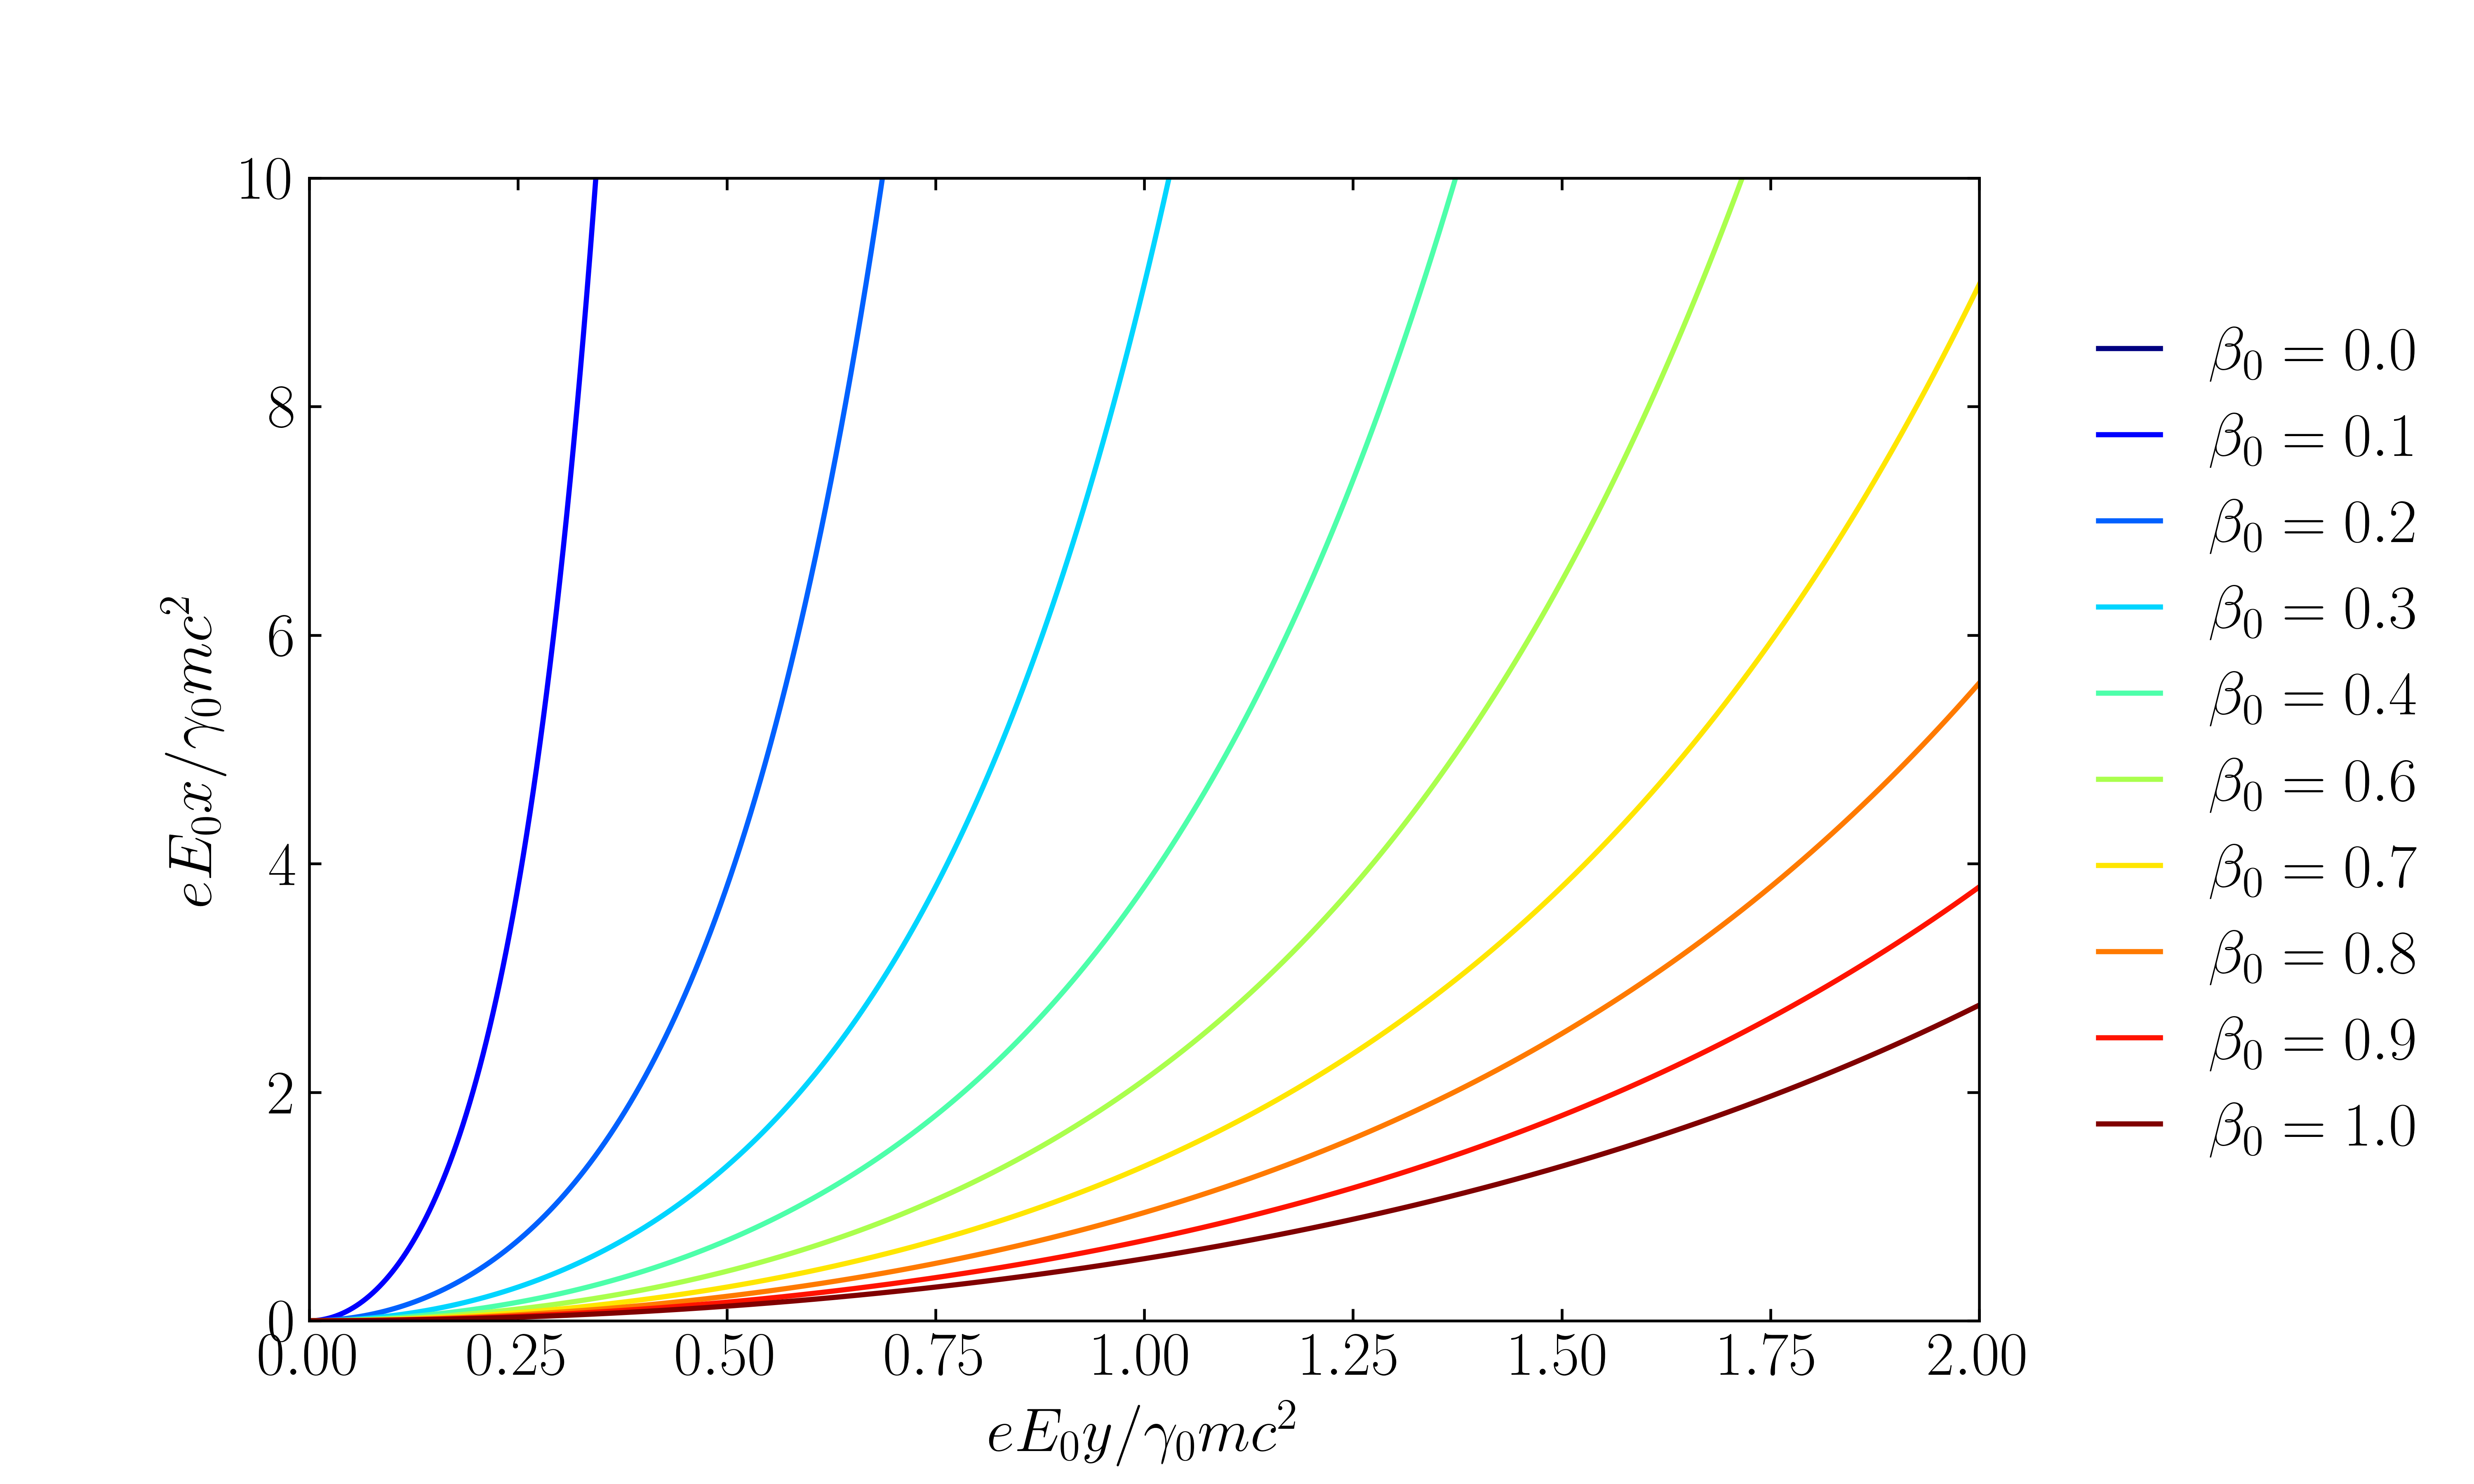
\includegraphics[width=\textwidth]{p1.png} 
\end{center}
Although the acceleration is along the electric field ($\xhat$), $u_y$
changes as $1/\gamma$ due to relativity, leading to a linear growth in $y$ in
proper time. However, $x$ grows exponentially. So $x$ increases faster than $y$
for a particle starting from rest $(u_{x0}=u_{y0}=0)$. For a relativistic
particle moving perpendicular to the field, this is the same, however, it takes
longer to steer it to point from $\yhat$ to $\xhat$. Here, short time means
$\overline{y}=eE_0y/\gamma_0mc^2\ll\beta_0$, while long time means 
$\overline{y}\gg\beta_0$. As soon as $\overline{y}$ grows past $\beta_0$, 
we observe significant change in $x$.
\end{solution}
\end{problem}
\newpage
%%%%%%%%%%%%%%%%%%%%%%%%%%%%%%%%%%%%%%%%%%%%%%%%%%%%%%%%%%%%%%%%%%%%%%%%%%%%%%%    
%%%%%%%%%%%%%%%%%%%%%%%%%%%%%%%%%%%%%%%%%%%%%%%%%%%%%%%%%%%%%%%%%%%%%%%%%%%%%%%
\begin{problem}{9.2}[Electric and magnetic fields at an angle]
Static, uniform electric and magnetic fields, $\vb{E}$ and $\vb{B}$, make an
angle of $\theta$ with respect to each other.

(a) Show that a Lorentz transformation can be made to go to a frame where
$\vb{E}'$ and $\vb{B}'$ are parallel, and that the boost velocity satisfies the
equation
\begin{equation}\label{p2a:beta}
    \frac{\bm\beta}{1+\beta^2}=\frac{\vb{E}\times\vb{B}}{E^2+B^2}. 
\end{equation}
\textit{Hint}: You can start with the trial solution
$\bm\beta=\lambda(\vb{E}\times\vb{B})$ and then show there is a $\lambda$ that
works.

(b) For $\vb{E}$ and $\vb{B}$ parallel, show that with appropriate constants of
integration, etc., the parametric solution can be written
\begin{equation}
    x=AR\sin\phi,\qquad
    y=AR\cos\phi,\qquad
    z=\frac{R}{\rho}\sqrt{1+A^2}\cosh(\rho\phi),\qquad
    ct=\frac{R}{\rho}\sqrt{1+A^2}\sinh\qty(\rho\phi),
\end{equation}
where $R=(mc^2/eB),\rho=E/B$, $A$ is an arbitrary constant, and $\phi$ is the
parameter (actually $c/R$ times the proper time).
\begin{solution}
(a) Let $\bm\beta=\lambda(\vb{E}\times\vb{B})$, as hinted. Then the transformed
fields are
\begin{equation}
    \vb{E}'=\gamma\qty[(1-\lambda
    B^2)\vb{E}+\lambda\qty(\vb{E}\vdot\vb{B})\vb{B}],
\end{equation}
and
\begin{equation}
    \vb{B}'=\gamma\qty[(1-\lambda
    E^2)\vb{B}+\lambda\qty(\vb{E}\vdot\vb{B})\vb{E}].
\end{equation}
Since $\vb{E}'\times\vb{B}'=\bm0$, $\lambda$ has to obey the following relation
\begin{equation}
    \lambda^2(\vb{E}\vdot\vb{B})^2=(1-\lambda B^2)(1-\lambda E^2) 
    \Rightarrow\lambda^2E^2B^2\sin^2\theta-\lambda(E^2+B^2)+1=0.
\end{equation}
However, note that $\abs{\bm\beta}^2=\lambda^2E^2B^2\sin^2\theta$. Plugging this
into the above equation yields
\begin{equation}
    \lambda=\frac{1+\beta^2}{E^2+B^2}, 
\end{equation}
as desired. Thus, the boost velocity is given by \eqref{p2a:beta}.

(b) Now, dropping the prime, in the transformed frame, the field tensor is
\begin{equation}
    F^{\alpha\beta}=\mqty(0&0&0&-E\\0&0&-B&0\\0&B&0&0\\E&0&0&0). 
\end{equation}
Then, the force equation is
\begin{equation}
    \frac{dU^\alpha}{d\tau}
    =\frac{c}{R}\mqty(0&0&0&-\rho\\0&0&-1&0\\0&1&0&0\\\rho&0&0&0)
    \mqty(U^0\\-U^1\\-U^2\\-U^3)
    =\frac{c}{R}\mqty(\rho U^3\\U^2\\-U^1\\\rho U^0).
\end{equation}
Thus, the separate components of $U^\alpha$ follows the 
following differential equations
\begin{align}
    \frac{d^2U^0}{d\tau^2}&=\frac{c^2\rho^2}{R^2}U^0 &
    \frac{d^2U^1}{d\tau^2}&=-\frac{c^2}{R^2}U^1\\
    \frac{d^2U^3}{d\tau^2}&=\frac{c^2\rho^2}{R^2}U^3 &
    \frac{d^2U^2}{d\tau^2}&=-\frac{c^2}{R^2}U^2.
\end{align}
The general solutions to which are
\begin{subequations}
    \begin{align}
        U^0&=A\sinh\qty(\rho \phi)+B\cosh\qty(\rho\phi)\\
        U^1&=C\sin\phi+D\cos\phi\\
        U^2&=C\cos\phi-D\sin\phi\\
        U^3&=A\cosh\qty(\rho\phi)+B\sinh\qty(\rho\phi),
    \end{align} 
\end{subequations}
where $A,B,C,D$ are constants and $\phi=c\tau/R$. First, recall that
$U^0=c\gamma=cdt/d\tau$, we can integrate to get
\begin{equation}
    ct=\int d\tau U^0
    =\frac{R}{c\rho}\qty[A\cosh\qty(\rho\phi)+B\sinh\qty(\rho\phi)].
\end{equation}
Forcing $t(\phi=0)=0$, $A=0$ and we can rewrite $B\mapsto c\sqrt{1+A^2}$ so that
\begin{equation}
    ct=\frac{R}{\rho}\sqrt{1+A^2}\sinh\qty(\rho\phi), 
\end{equation}
for some arbitrary constant $A$. Then it follows that
$\gamma=\sqrt{1+A^2}\cosh(\rho\phi)$ and $\gamma
u_z=c\sqrt{1+A^2}\sinh\qty(\rho\phi)$. So
\begin{equation}
    z=\int d\tau\gamma u_z=\frac{R}{\rho}\sqrt{1+A^2}\cosh(\rho\phi).
\end{equation}
Now, letting $C=0$ so that the initial conditions match the desired ones. Then,
note that by definition,
\begin{equation}
    \gamma^2
    =\sqrt{1+\frac{(U^1)^2+(U^2)^2}{c^2}+\frac{(U^3)^2}{c^2}}
    =1+\frac{D^2}{c^2}+(1+A^2)\sinh^2(\rho\phi)
    =(1+A^2)\cosh^2(\rho\phi).
\end{equation}
We can then solve for $D=cA$. The $x$ and $y$ positions thus follow
\begin{equation}
    x=\int d\tau U^1
    =AR\sin\phi,\qquad\t{and}\qquad
    y=\int d\tau U^2=AR\cos\phi.
\end{equation}
Note that to get these solutions, we had to assume $t(\tau=0)=0$ and $C=0$. So
these aren't general solutions.
\end{solution}
\end{problem}
\newpage
%%%%%%%%%%%%%%%%%%%%%%%%%%%%%%%%%%%%%%%%%%%%%%%%%%%%%%%%%%%%%%%%%%%%%%%%%%%%%%%
\end{document}
